\documentclass[12pt]{article} %Tipo de documento 
\usepackage[utf8]{inputenc} % Signos ortográficos del español 
\usepackage{amsmath} % Ecuaciones, símbolos y entornos matemáticos para ecuaciones y fórmulas
\usepackage{amssymb} % Ecuaciones, símbolos y entornos matemáticos para ecuaciones y fórmulas
\usepackage{graphicx} % Imágenes 
\usepackage[spanish]{babel} % Diseño de tablas (con opciones para la edición de otros gráficos)
\title{\textbf{Estructuras Discretas} \\
    {Práctica 2: Circuitos}}
\author{\textbf{Bonilla Reyes Dafne} \\ \\
    Facultad de Ciencias, UNAM}
\date{} 
\addtolength{\hoffset}{-2.5cm}
\addtolength{\textwidth}{5cm}
\addtolength{\voffset}{-2.5cm}
\addtolength{\textheight}{5cm} 
\graphicspath{{reporte/}}
\begin{document}
\maketitle
    \begin{enumerate}

        \item Diseña un circuito en el que calcule la suma de dos números 
            conformados por tres bits $x = x_2 x_1 x_0$ y $y = y_2 y_1 y_0$
            usando half-adders y full-adders.
            \\
            \\ 
            \textbf{Circuito:}
            \begin{figure}[h!]
                \centering 
                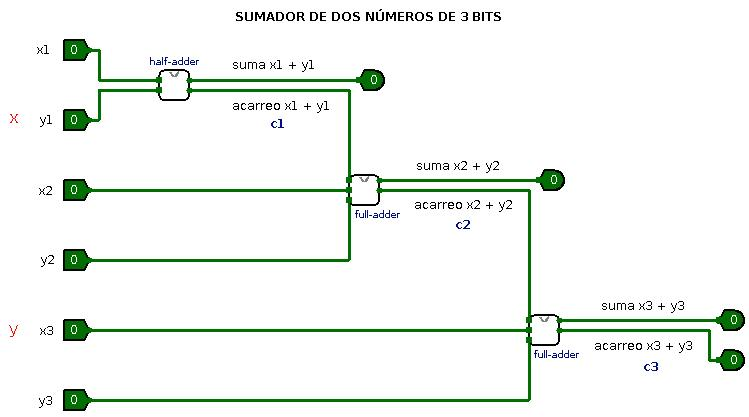
\includegraphics[scale=0.6]{ejercicio1.jpg}
                \caption{Circuito para la suma de dos números de 3 bits}
            \end{figure}
            \\
            \textbf{Justificación:} 
            Para crear este circuito, se parte de la idea intuitiva de 
            la suma tradicional de 2 números de 3 bits, para la cual se 
            suman dos bits por columna, llevando el bit de acarreo a 
            la siguiente, en donde se sumarán otros dos bits más el 
            de acarreo de la columna anterior, esto último dos veces. \\
            Por lo tanto, se crea un half-adder que recibe los datos de la 
            primera suma (dos bits sin contar el acarreo), y a continuación 
            dos full-adder que harán las siguientes dos sumas (reciben dos 
            bits más el bit de acarreo).\\
            Finalmente, se indica a que parte de la suma correspone cada 
            fragmento del circuito y el valor de la suma final indicada por
            las salidas con marca "suma".
            \\

        \item Diseña un circuito que controle la puerta de un elevador que
            está en un edificio de tres pisos. El circuito tiene 4 entradas. 
            $M$ es una señal lógica que está evaluada a 1 cuando el elevador se
            está moviendo. $F_1$, $F_2$, y $F_3$ son indicadores de que están 
            en ese piso. Por ejemplo, cuando el elevador está en el segundo
            piso, $F_2 = 1$ y $F_1 = F_3 = 0$.
            La salida del circuito es la señal que indica que la puerta se 
            abrirá, para que esto sucede, el elevador tiene que estar en 
            determinado piso y no se está moviendo. Da la tabla de verdad que
            describe el problema, encuentra la fórmula booleana en su FND, 
            minimízala con mapas de Karnaugh y haga el circuito correspondiente
            en logisim. 
            \\

            \textbf{Tabla de verdad:}
            \begin{table}[h!]
                \centering
                \begin{tabular}{|c|c|c|c|c|}
                    \hline
                    M & $F_1$ & $F_2$ & $F_3$ & Salida\\
                    \hline
                    1 & 0 & 0 & 0 & 0\\
                    \hline
                    0 & 1 & 0 & 0 & 1\\
                    \hline
                    0 & 0 & 1 & 0 & 1\\
                    \hline
                    0 & 0 & 0 & 1 & 1\\
                    \hline
                \end{tabular}
            \end{table}
        \\
        Para la tabla de verdad se dan los datos conocidos del problema, 
        en donde M se evalúa a 1 cuando el elevador está en movimiento, 
        es decir, no se encuentra en algún piso concreto, y una salida 1 
        cuando el elevador si se encuentra en un piso determinado y la puerta se abrirá.
        \\

        \textbf{FND: $M'F_1F_2'F_3' + M'F_1'F_2F_3' + M'F_1'F_2'F_3$}\\
        \\
        %Mapa de Karnaugh 
        \textbf{Mapa de Karnaugh:}
            \begin{figure}[h!]
                \centering 
                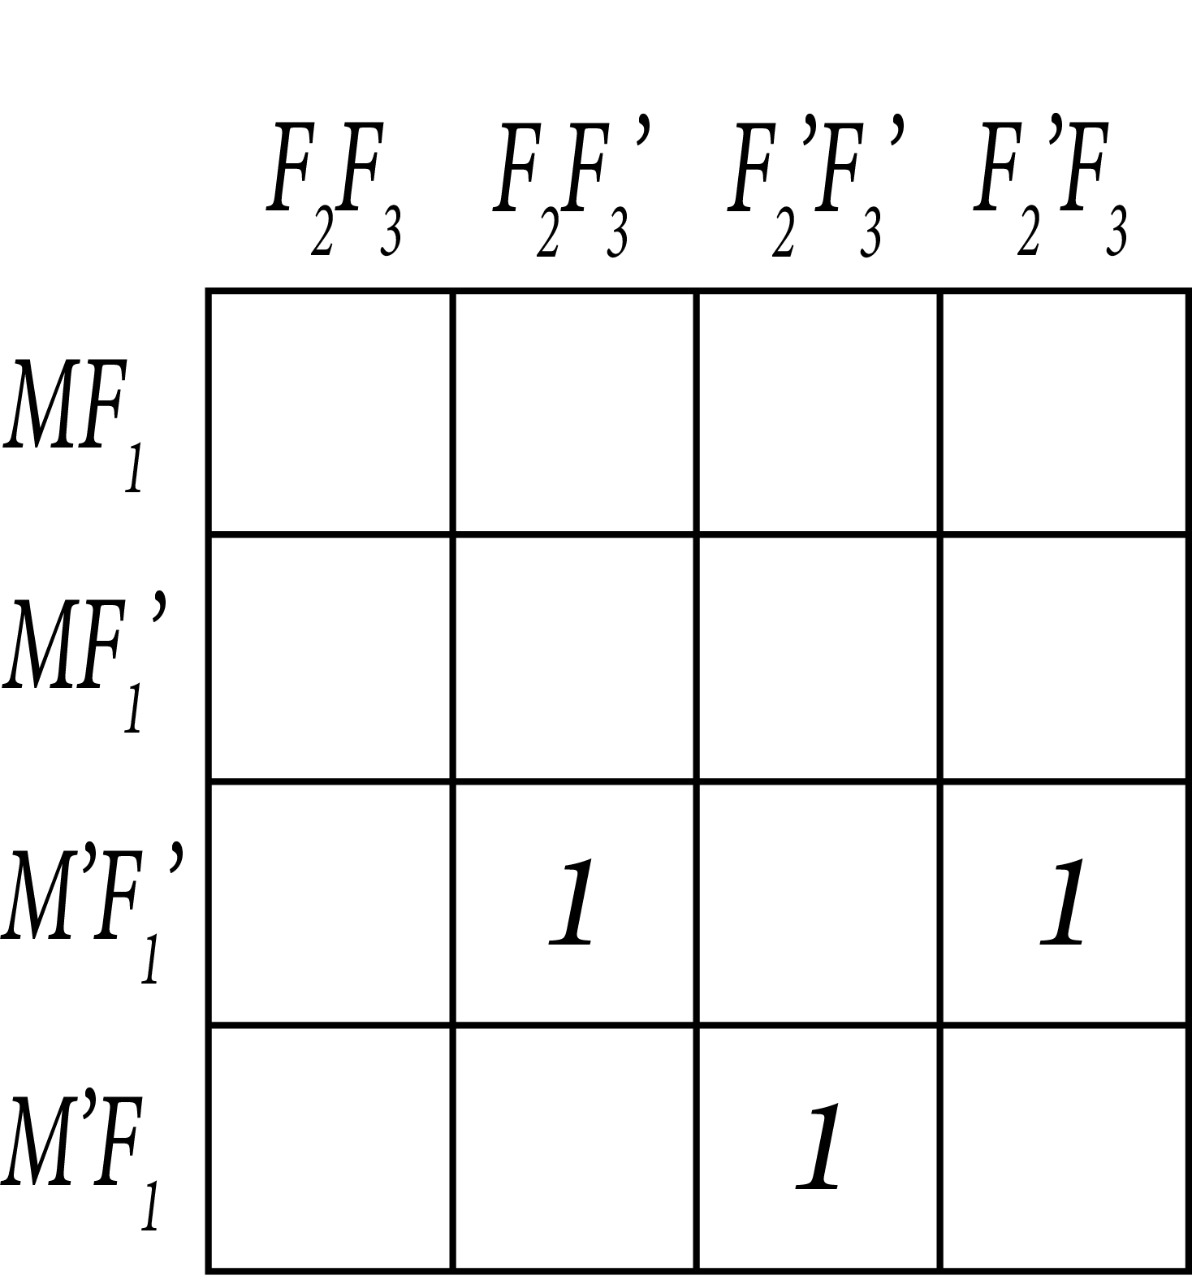
\includegraphics[scale=0.15]{Mapa1.jpeg}
            \end{figure}
        \\

        La minimización de una expresión booleana en su FND usando el 
        mapa de Karnaugh funciona a partir del encuentro de dos 
        mintérminos adyacentes, ya que cuando es el caso, podemos 
        minimizarlos y dar una expresión más simple. En este caso 
        ninguno de los mintérminos es adyacente a otro, por lo que la 
        expresión no se puede minimizar.
        
        \newpage 
        \textbf{Circuito:}
            \begin{figure}[h!]
                \centering 
                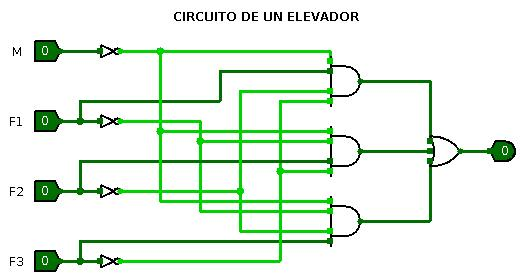
\includegraphics[scale=0.7]{ejercicio2.jpg}
                \caption{Circuito para un elevador}
            \end{figure}
        
        Finalmente, se da el circuito combinatorio para este problema,
        dando como entradas la señal $M$ y los 3 pisos del elevador. La
        salida de este circuito es 1 únicamente cuando el elevador se
        encuentra en un piso, no está en movimiento y la puerta se abre. 
        \\

        \item Escribe la expresión booleana para el siguiente circuito. 
            Diseña un circuito más simple. Justifique su respuesta.
            \begin{figure}[h!]
                \centering 
                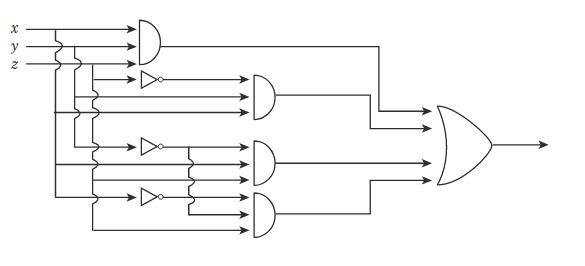
\includegraphics[scale=0.8]{circuito.jpg}
            \end{figure}
            \\
            \textbf{Expresión booleana en su FND:} $xy + y'z$ 
            \\

            \textbf{Justificación:} Para todo circuito combinatorio se 
            tienen valores de entrada, compuertas lógicas y valores de 
            salida. En este circuito se tiene a $x$, $y$ y $z$ como 
            valores de entrada, tres tipos de compuertas lógicas, AND, 
            OR y NOT, y finalmente un valor de salida. \\
            Al inicio tenemos 4 productos AND (algunos con el complemento 
            de un valor), dados en orden como:
                \begin{itemize}
                    \item 1. $xyz$
                    \item 2. $xyz'$
                    \item 3. $xy'z$
                    \item 4. $x'y'z$
                \end{itemize}
            A continuación, tenemos un OR, inidicando la suma de los 4 
            productos anteriores, por lo que tenemos la siguiente 
            expresión:
            
                \begin{center}
                    \textbf{{$xyz + xyz' + xy'z + x'y'z$}}
                \end{center}

            \textbf{Minimización de la FND:}
            Por mapa de Karnaugh y álgebra podemos obtener la minimización 
            de la expresión. 
                \begin{figure}[h!]
                    \centering 
                    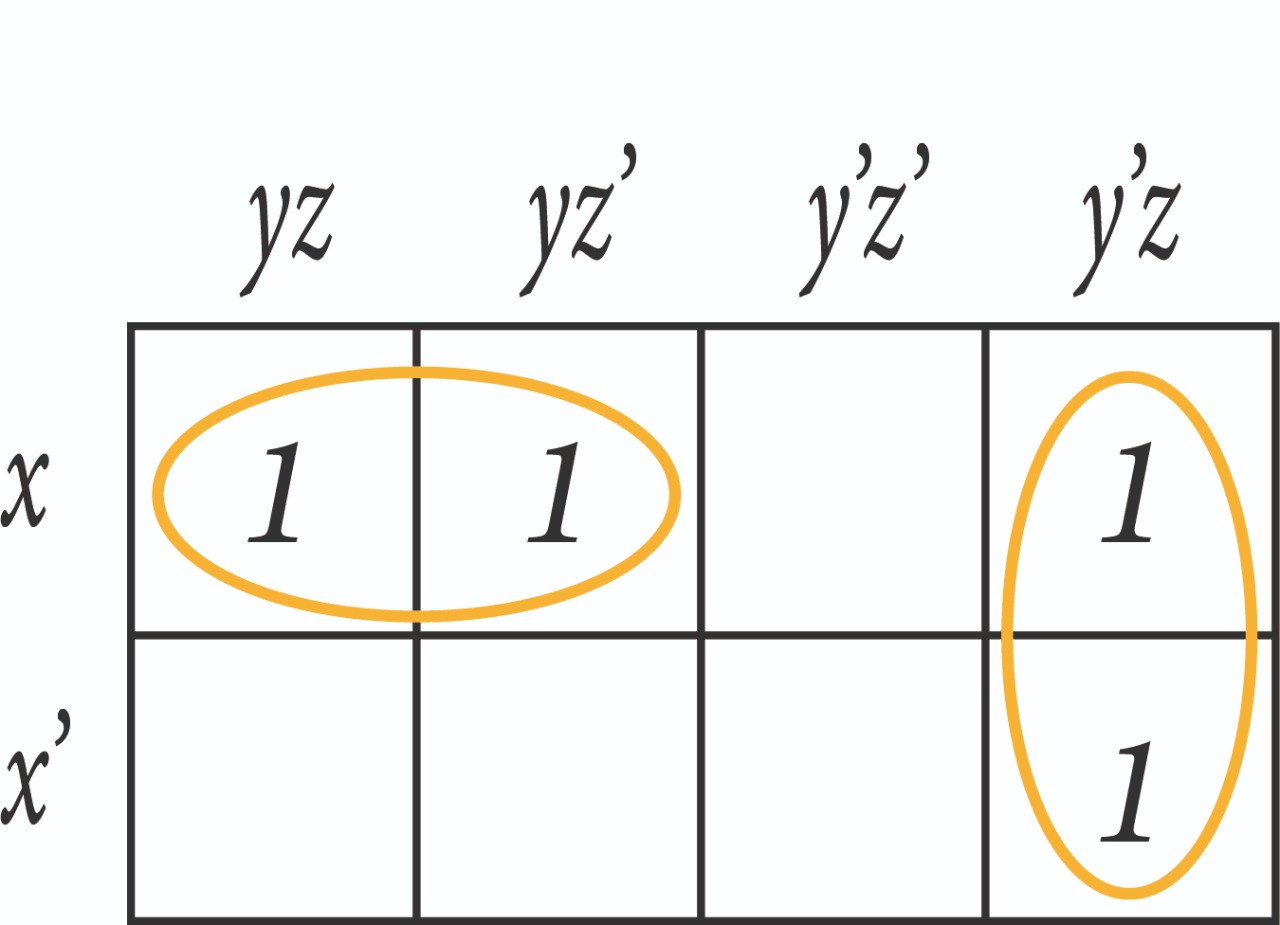
\includegraphics[scale=0.2]{Mapa2.jpeg}
                \end{figure}
            \\
            
            Para este mapa de Karnaugh tenemos el encuentro de dos pares de
            mintérminos adyacentes, por lo que podemos dar un expresión
            más simple. 
            \\

            Por lo tanto tenemos que:

            $xyz + xyz' + xy'z + x'y'z$ \\
            = $xy(z + z') + y'z(x + x')$ \\
            = $xy1 + y'z1$ \\
            = $xy + y'z$
            \\

            Entonces, la expresión booleana final en su FND es
            \textbf{{$xy + y'z$}}
            
            \newpage
            \textbf{Circuito:} 
            \begin{figure}[h!]
                \centering 
                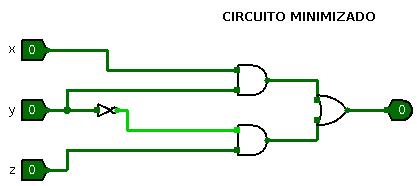
\includegraphics[scale=0.8]{ejercicio3.jpg}
                \caption{Circuito minimizado}
            \end{figure}
            \\
            Finalmente, damos el circuito para el problema a partir 
            de la expresión booleana minimizada obtenida, en donde 
            tenemos a $x$,$y$ y $z$ como entradas y un valor de salida
            que equivalente al del circuito original.
            \\

        \item Las cajas fuertes de los bancos usan diferentes tipos de candados 
            para prevenir cualquier acceso no autorizado. Un banco mejora su 
            seguridad mediante el uso de un candado combinatorio que funciona 
            con un sistema eléctrico,permitiendo que el candado se active o 
            desactive electrónicamente. Cuando está desactivado, la caja fuerte
            no se abrirá, incluso si la combinación usada es correcta. El candado
            de combinación es activado cuando dos apagadores, localizados en dos
            habitaciones separadas, son presionados. Además, para prevenir el 
            acceso cuando el banco está cerrado, incluso si la combinación de la 
            caja fuerte ha sido robada, un candado de tiempo es usado. Esto 
            significa que el candado de combinación solo está activado cuando el
            candado de tiempo también lo está. Diseña el circuito requerido para 
            determinar cuándo se puede acceder a la caja fuerte.\\
            
            \begin{figure}[h!]
                \centering 
                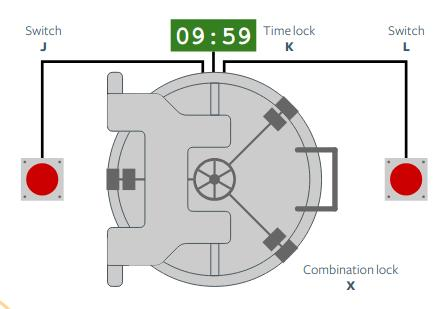
\includegraphics[scale=0.7]{caja.jpg}
            \end{figure}
            \newpage
            Para dar el circuito requerido primero damos la tabla de verdad
            que facilita la obtención de la FND para este problema. 
            \\

            \textbf{Tabla de verdad:} 
            \begin{table}[h!]
                \centering
                \begin{tabular}{|c|c|c|c|}
                    \hline
                    J & L & K & X \\
                    \hline
                    1 & 1 & 1 & 1 \\
                    \hline
                    1 & 1 & 1 & 0 \\
                    \hline
                    1 & 1 & 0 & 0 \\
                    \hline
                    1 & 1 & 0 & 0 \\
                    \hline
                    0 & 0 & 1 & 1 \\
                    \hline
                    0 & 0 & 1 & 0 \\
                    \hline
                    0 & 0 & 0 & 0 \\
                    \hline
                    0 & 0 & 0 & 0 \\
                    \hline
                \end{tabular}
            \end{table}
            \\
            Dada la tabla de verdad, tenemos que la caja fuerte se abre 
            en dos casos: cuando los apagadores y el candado de tiempo
            son activados o cuando solo el candado de tiempo es activado. 
            
            Por lo tanto, tenemos una expresión booleana en su FND como:
            \begin{center}
                $JLK + J'L'K$
            \end{center}

            \textbf{Circuito:} 
            \begin{figure}[h!]
                \centering 
                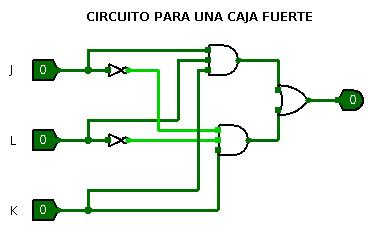
\includegraphics[scale=0.8]{ejercicio4.jpg}
                \caption{Circuito para una caja fuerte}
            \end{figure}
            \\
            Finalmente, tenemos un circuito combinatorio para el problema
            con 3 entradas que representan los dos apagadores y el candado
            de tiempo y una salida que indica cuando la caja fuerte se 
            abrirá.

    \end{enumerate}
\end{document}